\graphicspath{ {./images/} }
\chapter{設計}
\label{c:design}

無狀態區塊鏈為了縮減資料儲存空間,必須在交易附上證明,導致所需網路流量增大;
為了省去資料儲存裝置隨機存取所耗用的時間,必須花費 CPU 計算能力來驗證證明。

無狀態區塊鏈相較於一般區塊鏈做出了一些取捨(trade-off),
而淺狀態區塊鏈的目的是讓這種取捨不再是全有或全無(全部都附上證明或全部不附上證明),
使得狀態儲存的程度變得可調節。

\section{淺狀態區塊鏈}

無狀態區塊鏈中的一個區塊,如果多份交易的付款人、收款人都相同,
交易的證明也會是完全相同的,這樣重複的資訊顯然可以省略。

擴展這個想法,如果我們快取最近出現過的交易中的賬戶資訊,
則下一次收到同樣賬戶的交易時,也不需要去驗證證明。

再更進一步,讓整個網路上的節點都遵循同一套規則來記錄快取,
使得所有節點對於什麼時候要附證明、什麼時候不用附證明有共識,
那在區塊廣播的時刻,節點就能夠剝離掉不必要的證明,進而省下網路流量。

淺狀態相對於無狀態,犧牲了一些記憶體空間,但是只要存取快取的速度快過驗證證明的速度,
淺狀態區塊鏈就有望在效能上勝過無狀態區塊鏈。

% TODO: 補以太坊交易的快取分析圖

如果節點在驗證同一個區塊時,使用的快取不一致,
將會導致某些節點承認該區塊,某些節點不承認,從而導致分叉。

譬如,如果節點快取住它高度最高的 k 個區塊中的交易資訊,
當網路延遲,不同節點中的鏈分叉情形不同時,快取就會不一致,見下圖:

\begin{figure}[h]
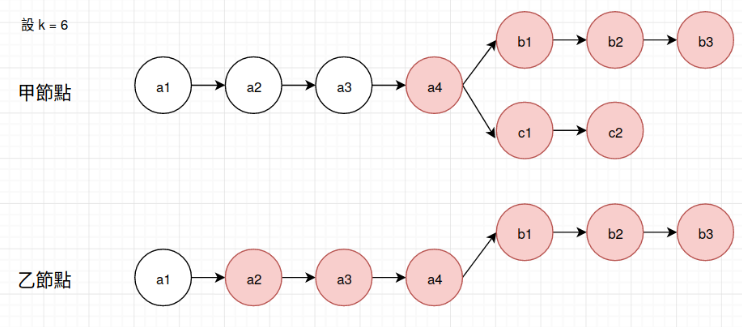
\includegraphics[width=\textwidth]{wrong-cache}
\caption{不一致的快取}
\end{figure}

粉紅色表示在快取,白色區塊表示不在快取。
此時若有一個不附證明的交易,付款方在 a2 區塊出現過,則乙節點會接收交易,甲節點則不會接收。

\section{快取設計}

一個簡單的設計準則可以避免前述的錯誤:每一個區塊都有自己的快取,
快取的內容僅僅由該區塊所在的鏈的資料所決定。
如此,我們把樹狀結構縮減為一個串列(list),
而不同節點上同個區塊所在的串列必定是相同的,
只要每個節點都用同樣的確定性演算法(deterministic algorithm)從這個串列計算出快取,
就能夠保證每個節點驗證同一個區塊時的快取一致。

\subsection{分叉處理}

觀察圖 3.2 中的鏈:

\begin{figure}[h!]
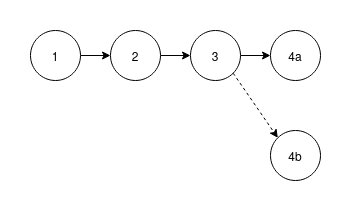
\includegraphics[width=10cm]{快取分叉}
\caption{區塊鏈分叉}
\end{figure}

此時,區塊 4b 嘗試接上區塊 3 ,因此它必須基於區塊 3 的快取來進行驗證。
也就是說,如果我們在接上區塊 4a 時,將區塊 3 的快取直接修改而稱為區塊 4a 的快取,
那當我們要街區塊 4b 時,就無從知悉區塊 3 的快取了,使用某些快取策略時,
我們可以透過回退(roll back)來取回區塊 3 的快取,但當使用某些快取策略時,遺失的快取無法輕易找回。

即使使用可以回退的快取策略,當分支切換越頻繁,回退的次數也會越頻繁,
回退的效能就可能就會成為瓶頸。

例如在圖 3.3 中,如果同時維持 a, b 兩條分支,則每次接收到非當前分叉的區塊時,都要進行回退,
並且隨著分叉的差異越大,回退的長度也越長,若從 7a 要走到 7b ,就必須先退回 3 ,再走回 7b ,
若之前曾經從 6a 走到過 6b ,則過程中的大部分運算都是相同的,這顯然是一種浪費。

\begin{figure}[h!]
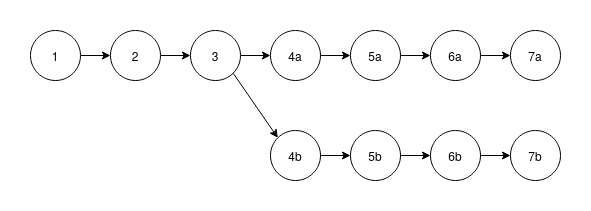
\includegraphics[width=\textwidth]{快取長分叉}
\caption{分叉頻繁切換}
\end{figure}

\subsection{持久化快取}

我們採用另外一種思路:在每個區塊上都保留它自己的快取,當新區塊要接上鏈的時候,
就可以直接取用它前一個區塊的快取,無需重新計算。
換句話說,我們採用全持久化資料結構(fully persistent data structure)~\cite{driscoll1986making}來儲存快取,
每接受一個區塊,就生成一個快取的版本。

在這個方案中,我們必須定時刪除太舊(例如,距離最長鏈超過 20 個區塊)區塊的快取,
以將整條鏈的快取大小限制在一定範圍,否則任由快取無限增長,將導致記憶體用罄,
以致於必須存取資料儲存裝置,快取就變得沒有意義了。

這個方案帶來了一個立即問題,如果我們每次都複製前一個區塊的快取,
那快取的所佔用的空間將會正比於未刪除的快取的數量。
然而,相鄰區塊中的快取有很高的相似性,若能選用適當的資料結構來讓相鄰區塊共享快取,
將能夠有效提高空間使用率。

\section{快取策略}

不同的快取策略在應對不同工作量(workload)時的命中率(hit rate)各不相同,
以下討論實作簡單的「最近 k 塊」策略,以及實作較為複雜,但經驗上命中率較高的 LRU 策略。

\subsection{最近 k 塊}

在「最近 k 塊」策略中,一個區塊的快取即為由該區塊開始,由高往低取 k 個區塊,
這 k 個區塊中出現過的交易中的資訊。

以下為 k = 6 的示意圖

\begin{figure}[h]
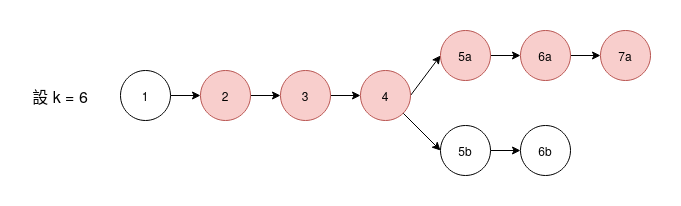
\includegraphics[width=\textwidth]{最近k塊}
\caption{區塊 7a 為粉紅色區塊中的所有交易資訊}
\end{figure}

可以用一個鍵值對(key value pairs)(其底層可為雜湊表(hash table)、平衡搜尋樹(balenced search tree)、跳躍鏈接串列(skip list)......等等)來表示快取,
若考慮每次重算的情境,例如在圖 3.4 中,要在 7a 區塊後接上一個 8a 區塊,
則我們加入 8a 區塊中的交易資訊,並丟掉只在 6a 中出現但沒有在其餘區塊中出現的交易資訊。

「最近 k 塊」的快取可以回退,跟前進時的演算法一樣,只是換了個方向。

當考慮全持久化時,我們可以選用可持久化的鍵值對資料結構,
例如雜湊\cite{bagwell2001ideal}\cite{puente2017persistence}、搜尋樹都有相對應高效成熟的持久化實作,
若一個快取有 n 個鍵,則持久化雜湊/搜尋樹插入/刪除一筆鍵值時,
時間、空間複雜度皆為 $O(log(n))$。

\subsection{LRU}

LRU 是 least recently used 的縮寫,這種策略中,快取大小是固定的,
若快取已滿,在插入新資料之前必須先丟棄一筆資料,
LRU 會去挑選快取中所有資料中最久沒被用到的那一筆來丟棄。

LRU 之所以比 FIFO 的命中率更高,是因為以太坊的歷史數據顯示,
(1) 一個賬戶花錢之後,很可能又接著花錢。 (2) 一個賬戶收到錢之後,
很可能會馬上將錢花掉。LRU 由於會更新資料的使用時間,得以一直快取住頻繁出現的資料,
FIFO 則只看資料進入快取的時間,只要快取失效會發生,
快取需要被抽換,那即使某些資料頻繁出現,遲早還是會被丟掉。

下表是 FIFO 跟 LRU 策略在不同快取大小時,
快取以太坊前一百萬個區塊中出現的賬戶所得到的命中率,
由此可以看出 LRU 在各種情況下都優於 FIFO 。因此我們優先研究 LRU 策略。

\begin{center}
\begin{tabular}{ | m{6em} | m{1cm}| m{1cm} | m{1cm} | m{1cm} | } 
\hline
快取賬戶數量& 10 & 100 & 1000 & 10000 \\ 
\hline
FIFO 命中率& 0.436 & 0.648 & 0.803 & 0.975 \\ 
\hline
LRU 命中率& 0.476 & 0.667 & 0.815 & 0.980\\ 
\hline
\end{tabular}
\end{center}


抽象來看, LRU 是一種支援兩個介面的資料結構,

\begin{itemize}
  \item get(key)
  \item put(key, value)
\end{itemize}

get(key) 時,若 LRU 存在該鍵,則返回對應值,並且將 key 的使用時間調整到最新。

put(key, value) 時,若 LRU 空間未滿,直接插入一筆鍵值對,
這筆新鍵值對的的使用時間為最新;若 LRU 空間已滿,
就要找出當前快取中使用時間最舊的丟掉,再插入新鍵值對,此新鍵值對的使用時間亦為最新。

對應到淺狀態區塊鏈的情境中,每當一個區塊要接上,我們要計算新區塊快取時,
會把一系列賬戶資訊的讀取跟修改操作轉變成 get 跟 put ,鍵是賬戶地址,值是賬戶狀態,
然後在 LRU 底層的資料結構上進行相應操作。

當在淺狀態區塊鏈中使用 LRU 策略時,是無法高效回退的。
當插入一筆鍵值對時,要丟棄的資料可能在好幾個區塊之外,
然而被修改的 LRU 無從得知這筆資料要去哪個區塊尋回。

\section{持久化 LRU 演算法}
在討論持久化 LRU 演算法之前,我們先觀察如何在軟體上高效實作 LRU 快取,
調查 github 上多個高使用量的 LRU 函式庫,內部資料結構都是雜湊表與雙向鏈表(doubly linked list)的組合:

\begin{figure}[h]
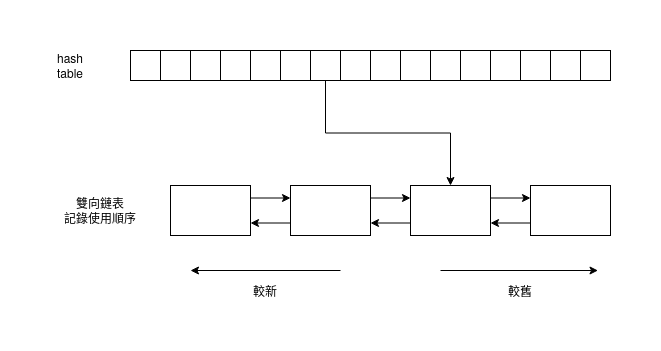
\includegraphics[width=\textwidth]{LRU}
\caption{LRU 資料結構}
\end{figure}

% TODO: 補圖

執行 get 時,透過雜湊得到指向節點的指標,獲取資料,並且將指標指向的鏈表節點移動至鏈表頭部(最左側)。
執行 put 時,若快取命中,更新節點的值,並將節點移動至鏈表頭部,
若快取未滿,從頭部加入快取值,並將其指標放入雜湊表,
若快取已滿,拔出雙向鏈表的尾部(最右側)節點,並且在雜湊表中移除該舊鍵,
然後在頭部加入快取值,放指標到雜湊表。

觀察到 LRU 需要記錄的資訊有二:

\begin{enumerate}
  \item 由鍵找到值(鍵值對)
  \item 各個鍵的順序資訊
\end{enumerate}

在前述的雜湊表 + 雙向鏈表的實現方案中,雜湊表負責 (1) ,雙向鏈表則負責 (2),
注意到,雙向鏈表極為自然的記錄了順序關係,它甚至不需要記錄確切的使用時間。

一個簡單的想法是,我們直接把雜湊跟雙向鏈表的持久化替代品組合起來,
就得到了一個持久化 LRU ,然而,雖然持久化雜湊有很成熟的替代品,
持久化雙向鏈表卻沒有。\footnote{
~\cite{driscoll1986making}提出了多種演算法能夠使得任何基於節點的資料結構半/全持久化(partial/fully persistent),
根據該論文的 node-splitting 演算法,
甚至能夠在 $O(1)$ 時間複雜度內完成雙向鏈表的插入、修改。

然而,該論文並沒有提出刪除持久化資料結構的老舊版本的方法,
這使得這些演算法難以應用到淺狀態區塊鏈的快取上,
因為無法刪除過去版本將導致快取所需的空間始終無法釋放,
最終耗盡記憶體容量。
}

因此,我們需要用其他可高效持久化的資料結構來取代雙向鏈表,進一步抽象雙向鍵表做的事情有:

\begin{itemize}
  \item 更新一個節點的使用時間到最新
  \item 刪除使用時間最舊的節點
  \item 插入新節點,新節點的使用時間為最新
\end{itemize}

以下,先討論了如何用紅黑樹\cite{guibas1978dichromatic}(平衡搜尋樹)來完成上述任務,
再介紹我們設計的順序樹(ordered tree)資料結構,相比紅黑樹,它更加高效。

\subsection{雜湊 + 紅黑樹}

我們嘗試使用紅黑樹來記錄順序資訊。首先,為每一筆賬戶資訊設置一個獨一無二的時間序,
這個時間序可以很容易得到,例如說設置成 $block\_height * max\_tx\_in\_one\_block + tx\_number$。

然後,以時間序做為鍵,賬戶資訊為值,建造一棵紅黑樹。雜湊表則用賬戶地址為鍵,對應的時間序為值。

get 時,先在雜湊表中由賬戶地址得到時間序,再到紅黑樹中由時間序得到賬戶資訊。
例如,在圖 3.6 中,我們會先從雜湊表得到賬戶的時間序為 243 ,再到紅黑樹中查找 243 。

\begin{figure}[h!]
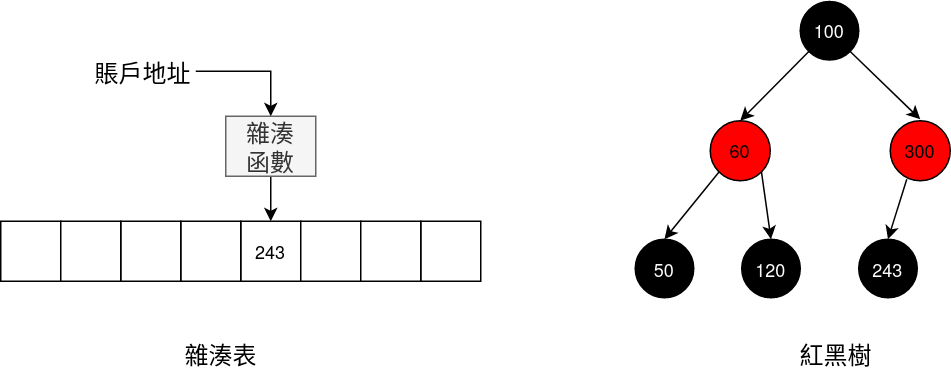
\includegraphics[width=\textwidth]{雜湊紅黑樹}
\caption{雜湊 + 紅黑樹}
\end{figure}

查找完成後,需更新使用時間。具體操作為修改雜湊表中地址對應的時間序,
並移除紅黑樹中的原節點,加入新時間序做為鍵。

put 類似於 get ,但需要修改賬戶資訊。

圖 3.6 表示不可變紅黑樹的共享結構。該圖中,快取的大小設為 8 。
狀態 1 時,只有 7 筆資料,狀態 2 對狀態 1 插入 14 ,資料變成 8 筆,
狀態 3 再對狀態 2 插入 15 ,由於快取已滿,必須先刪除時間序最小的資料,
也就是最左下角的紅色 7 。

\begin{figure}[h!]
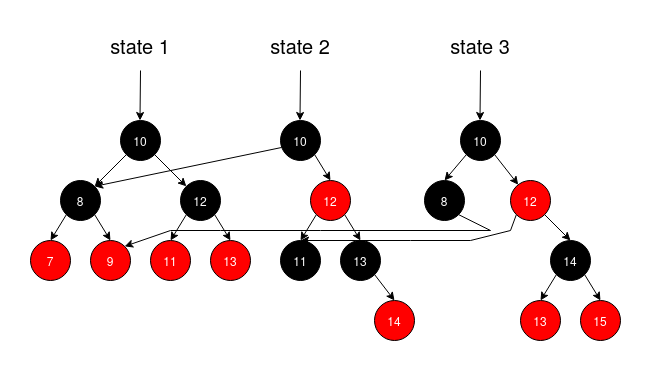
\includegraphics[width=\textwidth]{不可變紅黑樹}
\caption{不可變紅黑樹}
\end{figure}

% TODO:
% \subsubsection{紅黑樹 bulk 優化}

\subsection{雜湊 + 順序樹(ordered tree)}

雙向鏈接串列以節點之間的指向關係記錄順序關係,紅黑樹卻必須額外記錄時間序,
此外,原本透過雜湊就能一次查找到賬戶資訊,
紅黑樹方案卻得\emph{地址 -> 時間序 -> 賬戶資訊}兩段式地查找。

雙向鏈表無法以路徑複製來變換為不可變資料結構的原因在於,
兩個相鄰節點總是互指,一旦以路徑複製的方式修改節點,就得複製整個鏈表。
於是我們思考,不要用互指的方式來連接節點,就可以順利路徑複製。

想像在這些節點的背後編織一張網,然後將它們粘在一起(圖 3.8)。

\begin{figure}[h!]
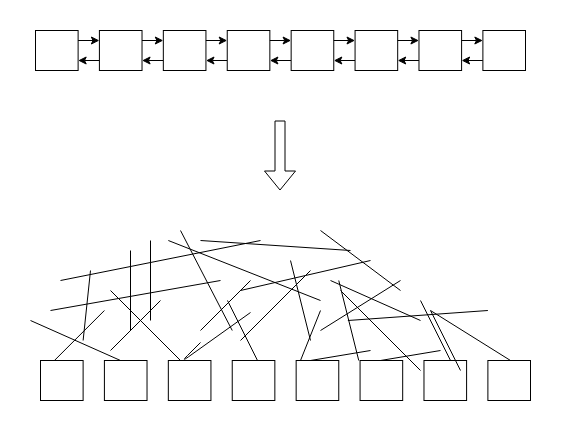
\includegraphics[width=\textwidth]{節點網}
\caption{以網連接節點}
\end{figure}

這個網狀結構最簡單形式就是一棵滿二元樹(full binary tree)(圖 3.9)。

\begin{figure}[h!]
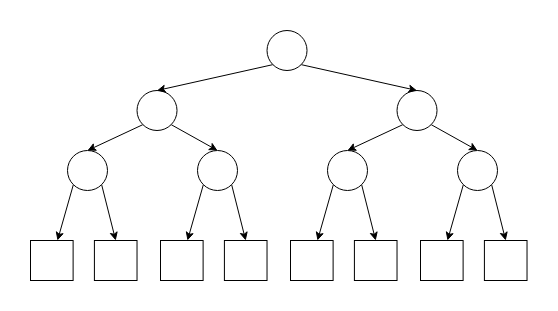
\includegraphics[width=\textwidth]{滿二元樹}
\caption{滿二元樹連接節點}
\end{figure}

我們將利用滿二元樹來儲存順序資訊的資料結構稱為順序樹,
以下開始一一介紹順序樹的各種操作。

若快取的容量為 $n$ ,順序樹的高度將會設置為 $1 + \lceil \log_2 n \rceil$,
也就是說,葉子的數量至少是快取容量的兩倍。圖 3.10 就是一棵容量為 4 的順序樹,它有 8 個葉子節點。

\begin{figure}[h!]
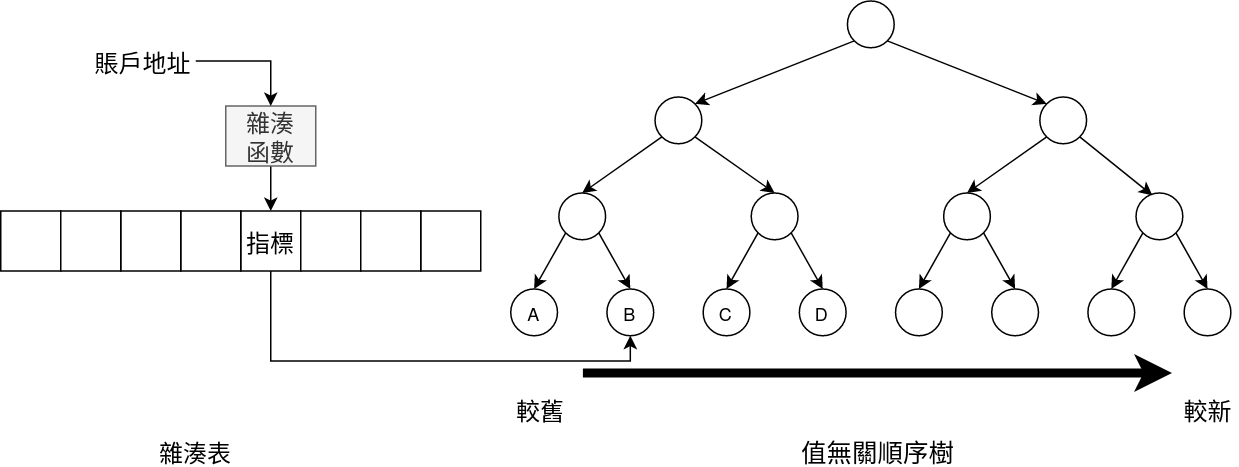
\includegraphics[width=\textwidth]{雜湊順序樹}
\caption{雜湊 + 順序樹}
\end{figure}

應用於 LRU 快取時,雜湊表所儲存的值會是一個指向順序樹葉子節點的指標,
只要一次雜湊表查詢就能取得資料。(見圖 3.10)

順序樹將所有資料都存放在葉子節點,每份資料按照使用時間的新舊來排列,
本文往後都按照資料越新,葉子的位置越右側的慣例來解釋跟畫圖。

順序樹的葉子有些有存放資料,有些沒有,我們將有存放資料的葉子稱為「有用葉子(used leaf)」,
沒有存放資料的葉子稱為「未用葉子(unused leaf)」。

get 時,將被查詢到的有用葉子改為未用的,並在當前最右有用葉子再往右一個的未用葉子中寫入原葉子的資料。
put 時,先找出最左側的有用葉子,將之改為未用的,並且在當前最右有用葉子再往右一個的未用葉子中寫入資料。

無論是 get 還是 put ,每次都會往右多佔用一個葉子,
如果當前最右的有用葉子已經在整棵樹的最右側了,就必須執行一次全複製,
把所有有用的葉子節點按照原本的順序緊密的排列在新順序樹的左側。

圖 3.11 演示了一連串的順序樹操作,其中狀態 7 到狀態 8 的時候發生了全複製。
圖中淺藍色節點表示它是未用的,注意到我們將所有葉子都未用的子樹的所有節點也都塗成淺藍了。

\begin{figure}[h!]
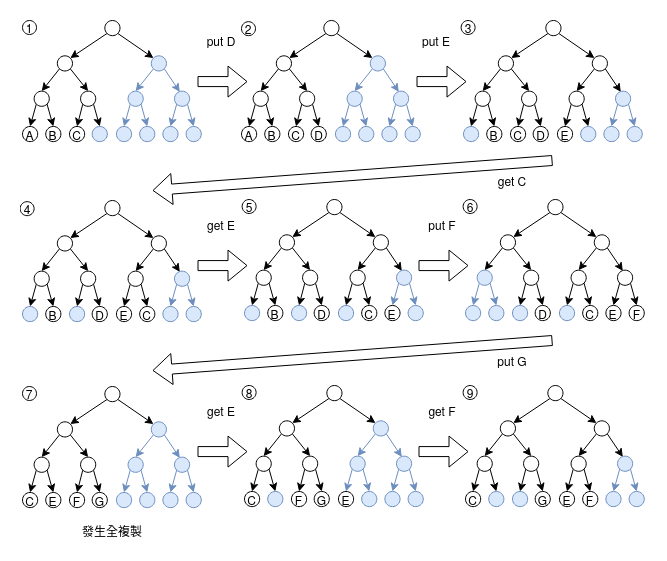
\includegraphics[width=\textwidth]{順序樹連續變化}
\caption{對順序樹進行一連串操作}
\end{figure}

在實作中,不需要真的為淺藍色節點分配記憶體空間,指向純淺藍色子樹的指標會是一個空指標(null pointer)。

\subsubsection{操作細節}

我們再接著探討 get, put 的操作細節。

要如何找出最左側的有用葉子?
從根部開始往下,若左側子節點非空,往左走,若左側子節點為空,往右走,走到高度為零時,就走到最左側有用葉子了。

從雜湊表中得到有用葉子的指標時,要如何知道該葉子在順序樹中的位置,以刪除它?
在葉子節點中,會儲存一個序號表示自己是從左到右的第幾個葉子,刪除葉子時,會從根一路往下,
判斷 $index \& (1 << height)$ 是否為 0 來決定往左還是右。

\subsubsection{時空間複雜度分析}

以下分析中,順序樹容量皆為 $n$ 。

若沒有發生全複製,get, put 都從根到葉子兩次,順序樹的高度是 $O(\log n)$,
時空間複雜度都是 $O(\log n)$。

如果發生全複製,就得遍歷一次順序樹,將所有有用葉子集結建一棵新樹,
注意到滿二元樹的總節點數量是葉子數量 * 2 - 1,不會超過 $n * 8$ ,
因此全複製的時空間複雜度是 $O(n)$ 。

$O(n)$ 的複雜度似乎有點高,但是每一次的 get/put 操作都只會讓有用葉子往右走一格,
一棵樹至少要 n 次操作,才會使有用葉子走到整棵樹的最右側。
順序樹是持久化資料結構,會同時維護多個版本,若每次在所有版本中選擇一個版本修改,
那平均要修改 n 次以上,才會觸發一次全複製,
在這種情況下,把全複製的成本攤銷到每一次操作,時空間複雜度是 $O(1)$ ,
get, put 的時空間複雜度依然是 $O(\log n)$ 。

最壞的情況是,每次都選擇將要發生全複製的版本來進行修改,
如此每個 get, put 操作的時空間複雜度都會是 $O(n)$ ,
但在 PoW 共識的系統中,必須有足夠的算力才能製造出一個區塊,
惡意打擊特定一個節點所耗費的代價巨大,而收效甚微。此外,
不一定要等有用葉子走到整棵樹的最右側才進行全複製,可以將全複製的時間點隨機化,
使得惡意的對手難以確定一個節點全複製的時刻。

嚴格來說,一個葉子的佔用的空間是 $O(\log n)$ ,因為葉子必須記錄自己的序號,
而序號在二進位的長度與順序樹的高度相同。但這不影響前述的空間複雜度分析,
即使考慮這點,時空間複雜度依然是 $O(\log n)$ 。
況且,實作中不可能會創建容量超過 CPU 定址空間大小的順序樹,
序號必定能用 64bit 的整數存下。